%%%% CAPÍTULO 2 - REVISÃO DA LITERATURA (OU REVISÃO BIBLIOGRÁFICA, ESTADO DA ARTE, ESTADO DO CONHECIMENTO)
%%
%% O autor deve registrar seu conhecimento sobre a
%% literatura básica do assunto, discutindo e 
%% comentando a informação já publicada. A revisão deve
%% ser apresentada, preferencialmente, em ordem
%% cronológica e por blocos de assunto, procurando
%% mostrar a evolução do tema.

%% Título e rótulo de capítulo (rótulos não devem conter caracteres especiais, acentuados ou cedilha)
\chapter{Hardware}\label{cap:Hardware}

O Hardware visa facilitar a interação entre o Usuário e o sistema, proporcionando um display para comandos ao controlador que realizará o controle de movimentação dos motores, as coletas dos dados do sensor a respeito dos pontos dos objetos e também o armazenamento desses dados através do módulo SD. 

\section{Eletrônica}

%tabela dos componentes com o preço
%explicação breve sobre cada um deles


O projeto de Hardware foi desenvolvido utilizando a ferramenta on-line \href{https://easyeda.com/}{EasyEDA}. Foi levado em consideração o uso de módulos para facilitar o desenvolvimento do projeto, sendo eles:

\begin{itemize}
    \item 1 Devkit Node MCU com Microcontrolador ESP32
    \item 2 Motores Nema 17
    \item 1 Sensor IR de distância GP2Y0A51SK0F
    \item 2 Controladores de servo motor modelos A4988 e DRV8825
    \item 1 Módulo para Leitura/Escrita de cartão SD
    \item Regulador 5V para alimentação dos componentes
    \item Fonte 12V 2A
    \item Conector P4 Femea para fonte de 12V
    \item Diodo para evitar erro de polarização da fonte
    \item Capacitores acopladores
\end{itemize}

\subsection{Devkit Node MCU ESP32}
O Devkit NodeMCU com microcontrolador ESP32 é uma plataforma de desenvolvimento popular para projetos de Internet das Coisas (IoT). Baseado no chip ESP32 da Espressif Systems, ele oferece um microprocessador dual-core com clock de até 240 MHz, conectividade Wi-Fi e Bluetooth integradas, e uma ampla gama de pinos de entrada e saída para diversas funções. A placa também inclui componentes úteis como regulador de tensão, portas USB para alimentação e programação, e botões de reset e boot, facilitando a prototipagem e desenvolvimento de projetos conectados.

\subsection{Motores Nema 17}
Os motores Nema 17 são motores de passo amplamente utilizados em aplicações que exigem controle preciso de movimento, como impressoras 3D, máquinas CNC e robótica. O "Nema 17" refere-se ao padrão de montagem da National Electrical Manufacturers Association, indicando que o motor possui uma face frontal de 1,7 polegadas (aproximadamente 43 mm). Esses motores geralmente oferecem um ângulo de passo de 1,8 graus, resultando em 200 passos por rotação completa, permitindo um controle detalhado e preciso da posição.

\subsection{Sensor IR de Distância}
O sensor GP2Y0A51SK0F é um sensor de distância infravermelho fabricado pela Sharp. Este sensor é conhecido por sua capacidade de medir distâncias de forma precisa e confiável em um intervalo de 2 cm a 15 cm. Utiliza um feixe infravermelho e um sensor de posição para detectar a presença de objetos e calcular a distância com base no ângulo de reflexão do feixe infravermelho.

O GP2Y0A51SK0F foi utilizado para a obtenção dos pontos do objeto. A saída analógica do sensor proporciona uma leitura proporcional à distância do objeto, o que simplifica a interface com microcontroladores e outros sistemas de controle.

\subsection{Controladores A4988 e DRV8825}
Os controladores A4988 e DRV8825 são drivers de motor de passo amplamente utilizados para controlar motores de passo em aplicações como impressoras 3D, máquinas CNC e robótica. Ambos são populares devido à sua eficácia, facilidade de uso e recursos avançados de controle.

\textbf{A4988}: O A4988 é um driver de motor de passo fabricado pela Allegro MicroSystems. É conhecido por sua simplicidade e capacidade de controle preciso de motores de passo. Algumas características principais incluem:

\begin{itemize}
    \item Microstepping: Suporta até 1/16 de microstepping, o que permite um controle de posição suave e preciso do motor.
    \item Corrente Ajustável: Possui um potenciômetro que permite ajustar a corrente de saída máxima, protegendo o motor contra sobrecorrente.
    \item Proteções Integradas: Inclui proteção contra sobrecorrente, sobretemperatura e undervoltage lockout.
    \item Interface Simples: Utiliza uma interface de passos e direção simples, facilitando a integração com microcontroladores e outros sistemas de controle.
\end{itemize}


\textbf{DRV8825}: O DRV8825 é um driver de motor de passo fabricado pela Texas Instruments, oferecendo recursos avançados e desempenho superior em comparação com o A4988. Suas características principais incluem:

\begin{itemize}
    \item Microstepping: Suporta até 1/32 de microstepping, proporcionando um controle de posição ainda mais suave e preciso do motor.
    \item Corrente Ajustável: Similar ao A4988, permite ajustar a corrente de saída máxima através de um potenciômetro.
    \item Proteções Integradas**: Inclui proteção contra sobrecorrente, sobretemperatura, undervoltage lockout e proteção contra curto-circuito.
    \item Capacidade de Corrente Maior: Pode fornecer até 2,5A por fase com refrigeração adequada, tornando-o adequado para motores de passo maiores e mais potentes.
    \item Interface Simples: Utiliza a mesma interface de passos e direção, facilitando a substituição direta do A4988 em muitos projetos.
\end{itemize}

\subsection{Módulo SD}

O módulo SD para ESP32 é uma interface que permite a comunicação entre o microcontrolador ESP32 e cartões de memória SD, oferecendo uma maneira eficiente de armazenar grandes volumes de dados. Esse módulo é frequentemente usado em projetos que necessitam de armazenamento de dados como registro de sensores, gravação de logs, armazenamento de arquivos de mídia, e mais. Possui as seguintes características:

\begin{itemize}
    \item Comunicação SPI: Utiliza a interface de comunicação Serial Peripheral Interface (SPI) para se conectar ao ESP32, garantindo uma comunicação rápida e eficiente.
    \item Compatibilidade: Suporta cartões SD e microSD, permitindo flexibilidade na escolha do meio de armazenamento.
    \item Bibliotecas: O ESP32 é compatível com várias bibliotecas de software, como a biblioteca SD da Arduino IDE, facilitando a integração e programação.
    \item Capacidade de Armazenamento: Suporta cartões de alta capacidade (HC) e de capacidade estendida (XC), permitindo armazenamento de dados em gigabytes.
\end{itemize}

\section{Esquematico Eletrônico}


\subsection{Esquema Eletrônico}
%foto do esquema eletrônico

O esquema eletrônico (Figura \ref{figura:esquema_eletonico }) foi desenvolvido utilizado a plataforma \href{https://easyeda.com/}{EasyEDA}.

\begin{figure}[H]
\captionsetup{width=0.6\textwidth}%% Largura da legenda
\caption{ Esquema Eletrônico }%% Legenda
\label{figura:esquema_eletonico }%% Rótulo
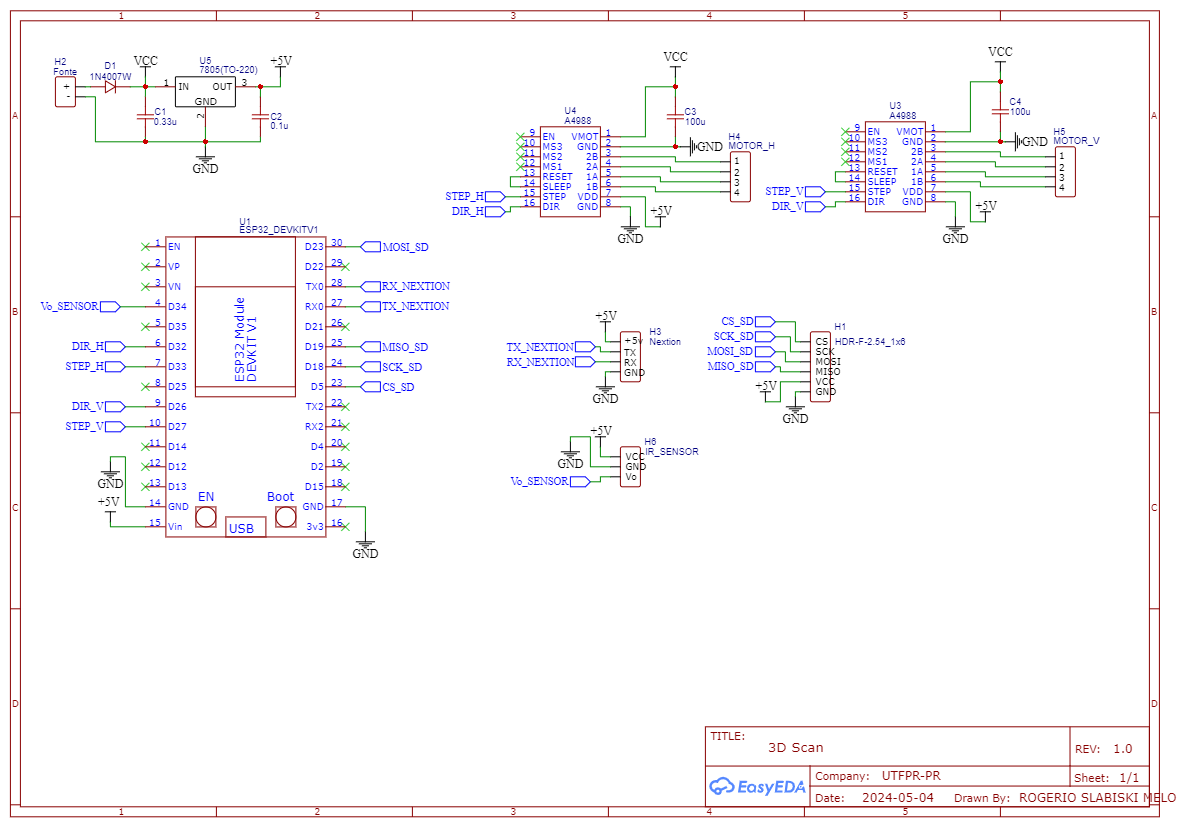
\includegraphics[width=0.85\textwidth]{3.Hardware/Imagens/esquematico-eletronico.png}%% Dimensões e localização
\fonte{AUTORES}%% Fonte
\end{figure}

\section{PCB}
%foto do pdf do pcb
%foto do pcb, as duas versões
%foto da placa universal

O projeto da placa PCB também foi desenvolvido utilizando a plataforma Easy EDA \cite{site:easyeda}, exibido na Figura \ref{figura:esquema_pcb}.

\begin{figure}[H]
\captionsetup{width=\textwidth}%% Largura da legenda
\caption{ Projeto do PCB }%% Legenda
\label{figura:esquema_pcb}%% Rótulo
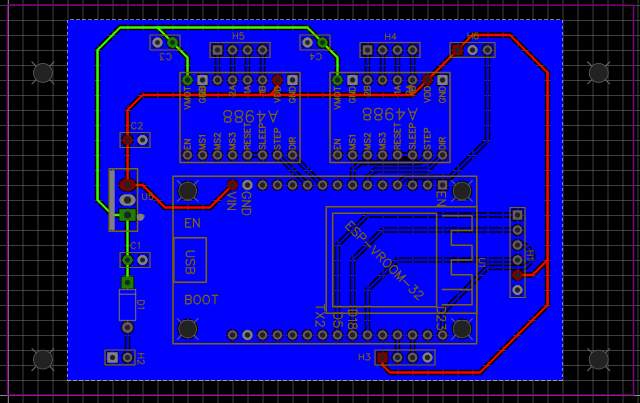
\includegraphics[width=0.9\textwidth]{3.Hardware/Imagens/esquema-pcb.png}%% Dimensões e localização
\fonte{AUTORES}%% Fonte
\end{figure}

\section{Implementação do Hardware}

A implementação do hardware foi desenvolvida através de uma placa universal, pois foi realizado o orçamento da fabricação industrial mas estourava o orçamento e o cronograma para a finalização do projeto.
As fotos a seguir apresentam a versão final da implementação:

\begin{figure}[H]
\captionsetup{width=\textwidth}%% Largura da legenda
\caption{ Hardware parte superior }%% Legenda
\label{figura:hardware_superior}%% Rótulo
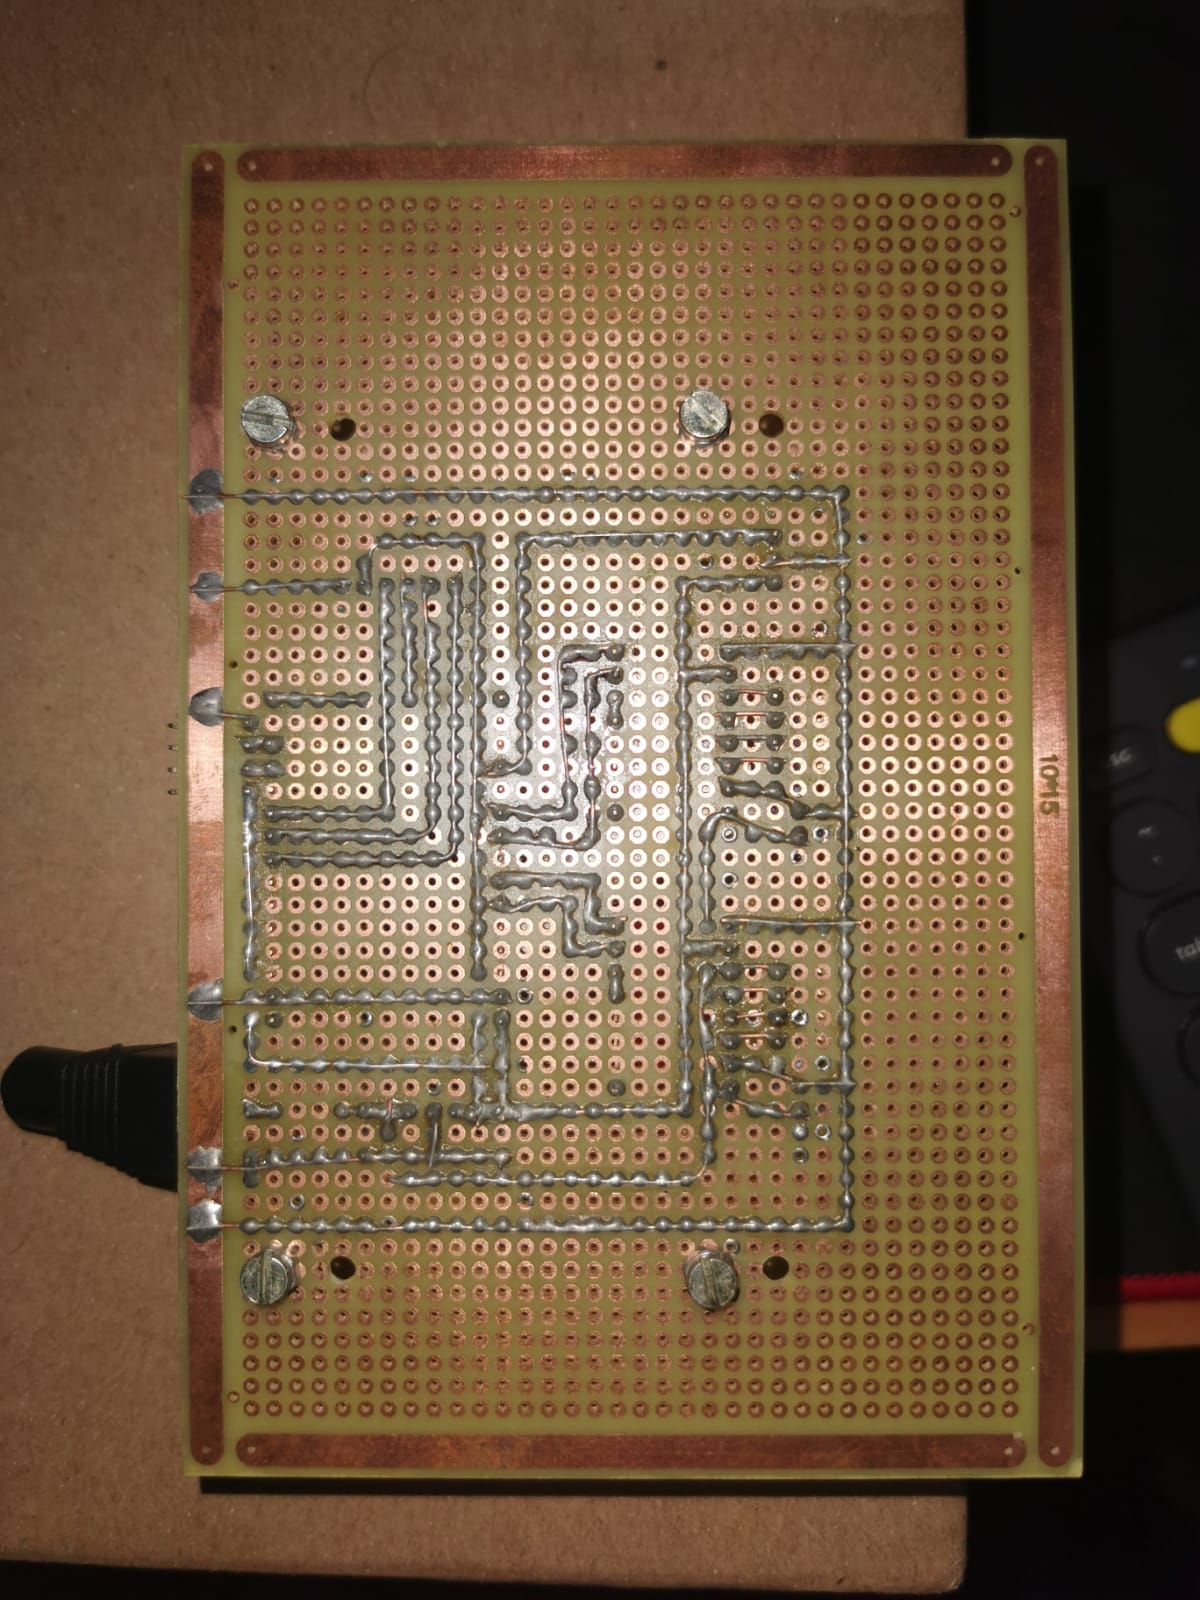
\includegraphics[width=0.9\textwidth]{3.Hardware/Imagens/hardware-01.jpeg}%% Dimensões e localização
\fonte{AUTORES}%% Fonte
\end{figure}


\begin{figure}[H]
\captionsetup{width=\textwidth}%% Largura da legenda
\caption{ Hardware parte inferior }%% Legenda
\label{figura:hardware_inferior}%% Rótulo
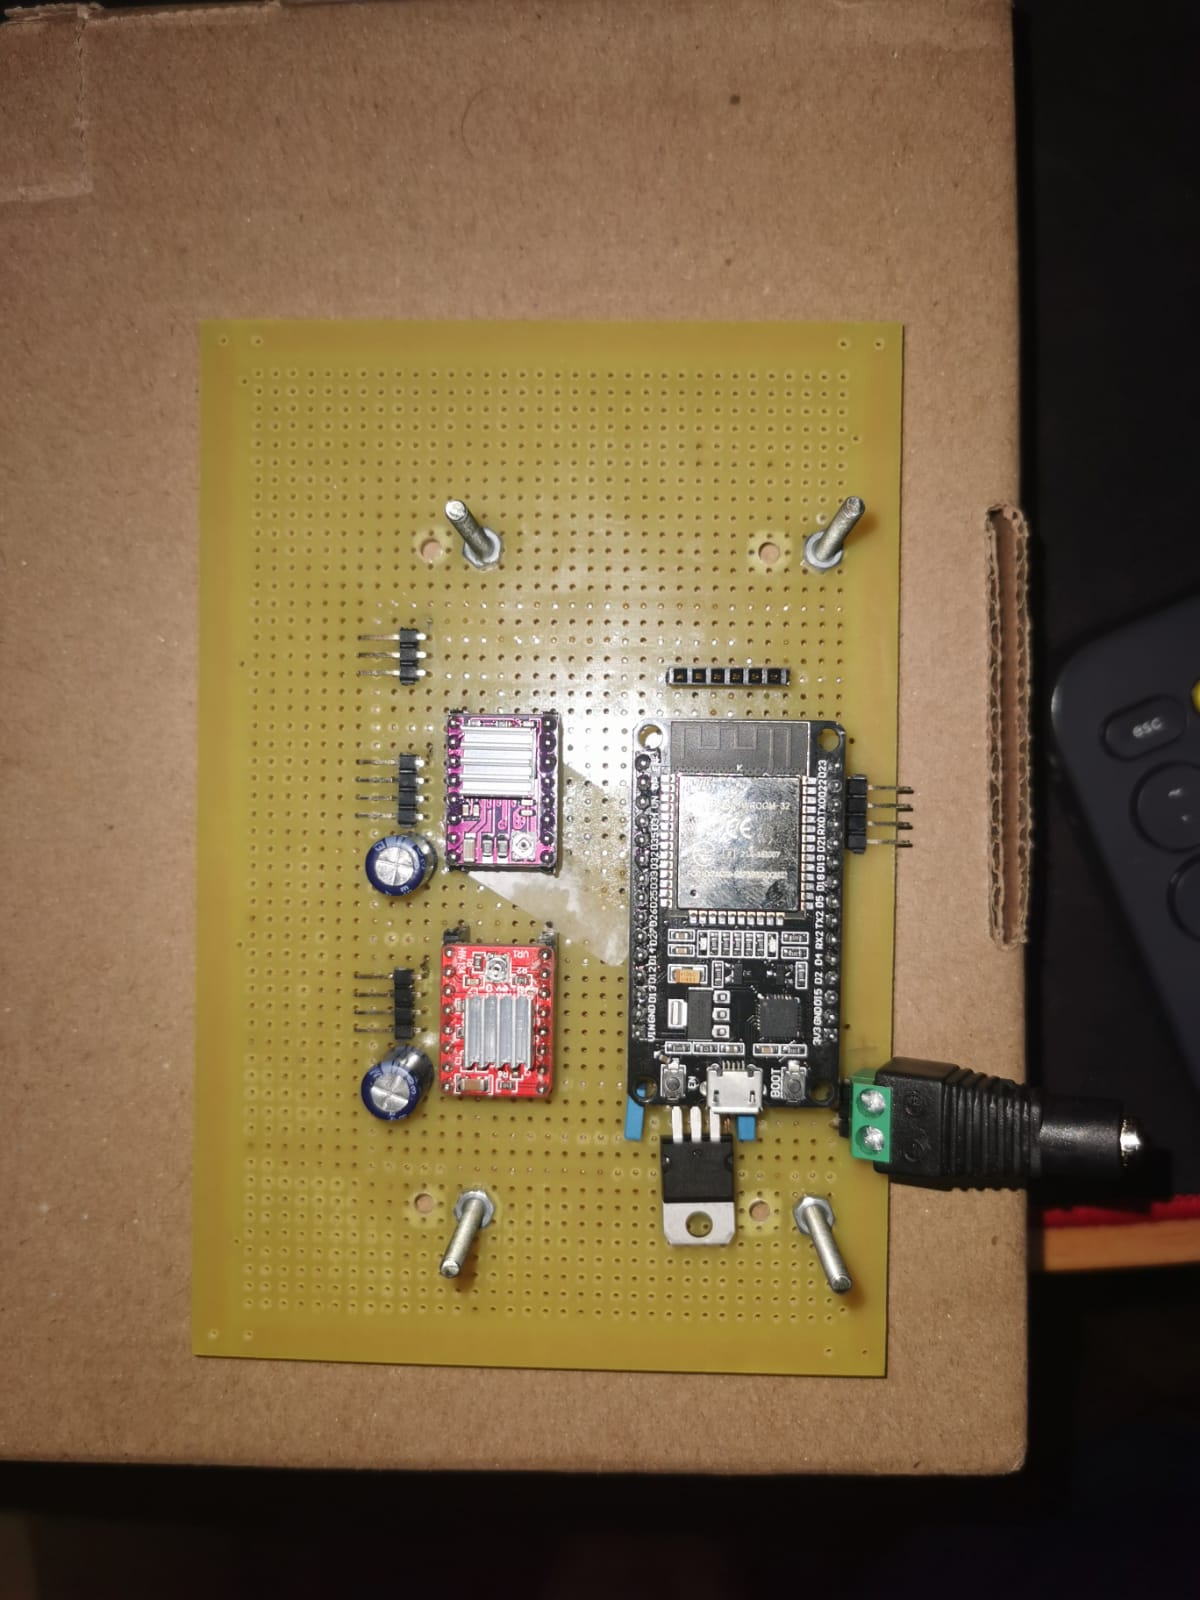
\includegraphics[width=0.9\textwidth]{3.Hardware/Imagens/hardware-02.jpeg}%% Dimensões e localização
\fonte{AUTORES}%% Fonte
\end{figure}